\label{sec:2.4}

%%%%%%%%%%%%%%%%%%%%%%%%%%%%%%%%%%%%%%%%%%%%%%%%%%%%%%%
% Lin and Prakash - LBL test setup
%%%%%%%%%%%%%%%%%%%%%%%%%%%%%%%%%%%%%%%%%%%%%%%%%%%%%%%

A single board solution was developed by LBNL to test the ColdADC. The mother board accommodates one ColdADC bare die, wire bonded to the board. The mother board is divided into ``cold" and ``warm" sections with an empty strip of PCB in between to clamp the board to CTS. The ColdADC, extremely low noise LDO's which supply four different VDDs to the ColdADC are present in the ``cold section" of the mother board. Power supply distribution circuitry, Spartna 6 FPGA, LDO's for the FPGA, 80MHz oscillator for clocking the FPGA, external unity buffers and 12 bit ADCs to digitize the monitor signals from the ColdADC and 40 pin standard header to connect the Raspberry PI are in the ``warm section" of the mother board. Analog inputs to the ColdADC are supplied by 16 edge-mount SMA connectors. There are two additional edge-mount SMA connectors to supply test inputs directly to the ADC-core. Eight-pin standard header connector is available if there is a need to bypass the ColdADC LDOs and supply external VDDs directly to the ASIC.

Although the mother board is very successful, there are three minor limitations: Due to small block-ram size of the FPGA the ADC data cannot be streamed continuously to the Raspberry PI this makes the calibration and linearity calculation of the ColdADC a time consuming process. Secondly, this version of the mother board is a Chip-On-Board (COB) version, this makes testing more than one ASIC very difficult, replacing an ASIC essentially means destroying the current chip and mount a new chip. Finally, the analog inputs to the ColdADC can only be single ended. Due to the lack of space only 16 SMA connectors were mounted on the board.  

A new three board solution was developed to overcome these three limitations. Version 2 LBNL test setup consists of a motherboard, a daughter card and an FPGA mezzanine board. The daughter card can either designed to have bare die or a packaged chip. A modular approach was taken to design the new test setup. The same test setup can be used for ColdADC V2 chip just by minor re-designing the COB daughter card. The V2 LBNL test setup is shown in Figure \ref{fig:v2_board}. This test board, just like the previous version has ``cold section" and ``warm section". The COB daughter card and the LDOs are at the bottom, in the ``cold" section of the board. The power distribution circuitry, FPGA mezzanine board, and the Raspberry PI are in the ``warm" section of the board. Four 8-pin Samtec 5.00 mm 50 Ohm Ganged Micro-Miniature RF Jack connectors are used to drive external differential or single ended analog inputs to the ColdADC.  

\begin{figure}[!ht]
\centering
  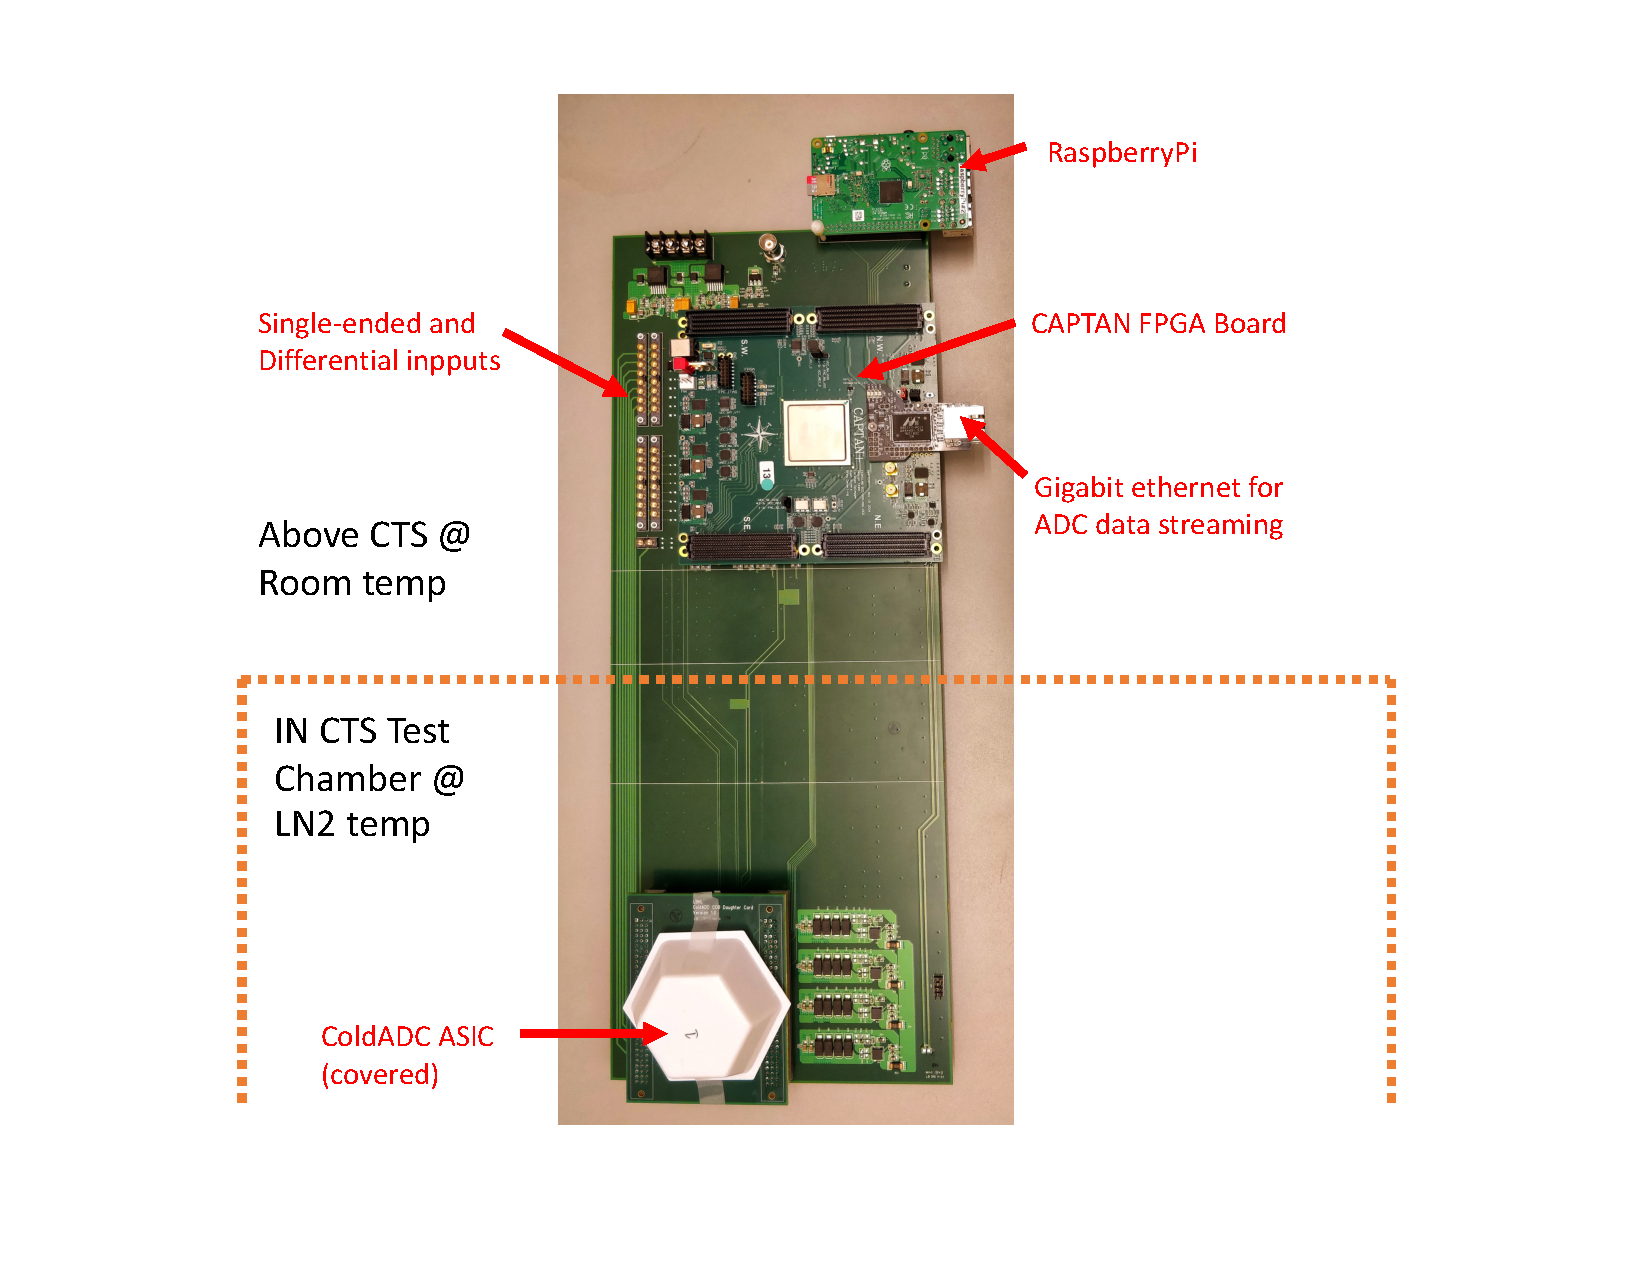
\includegraphics[width=0.85\linewidth]{figures/prakash_fig/TestBoard2_CTS.pdf}
  \caption[LBNL ColdADC Testboard]{Version 2 LBNL ColdADC Testboard}
  \label{fig:v2_board}
\end{figure}


